\documentclass{article}
\usepackage{amsmath}
\usepackage{amssymb}
\usepackage{hyperref}
\usepackage{xcolor}
\usepackage{graphicx}
\usepackage{hyperref}

\title{A Modest (Tokenomics) Proposal, Version 3}
\date{250324}
\author{}

\begin{document}

\maketitle

\section{Goals}\label{sec:goals}
\begin{itemize}
    \item HYPR provides genuine utility to users,
    \item HYPR has long-term incentives to keep demand in long-term,
    \item HYPR allows user to participate in useful DAO governance.
\end{itemize}

\section{Voting Power}\label{sec:votingpower}

Voting power depends on two parameters: $n$, the number of HYPR tokens locked, and $t$, the remaining period tokens are locked for (in weeks).
Token supply is denoted $S$ (it is $10^9$).
Max lock time is denoted $T$ (it is some small single-digit number of years).
The voting power of a wallet is denoted $V(n, t)$.
\begin{equation}
V(n, t) = (an - bn^2) \cdot (ct - dt^2)
\end{equation}

The parameters $a$, $b$, $c$, $d$, all greater than or equal to $0$, are chosen such that voting power is a strictly monotonically-increasing function of $n$ and $t$ (i.e. it only ever increases as $n$ and $t$ increase).
This leads to the following requirements for the parameters:
\begin{align}
a &> 2b \cdot n_m\\
c &> 2d \cdot T
\end{align}

where $n_m$ is the maximum number of tokens that a single wallet can lock.
$n_m$ can reasonably be set to $S$.

\begin{figure}[h]
    \centering
    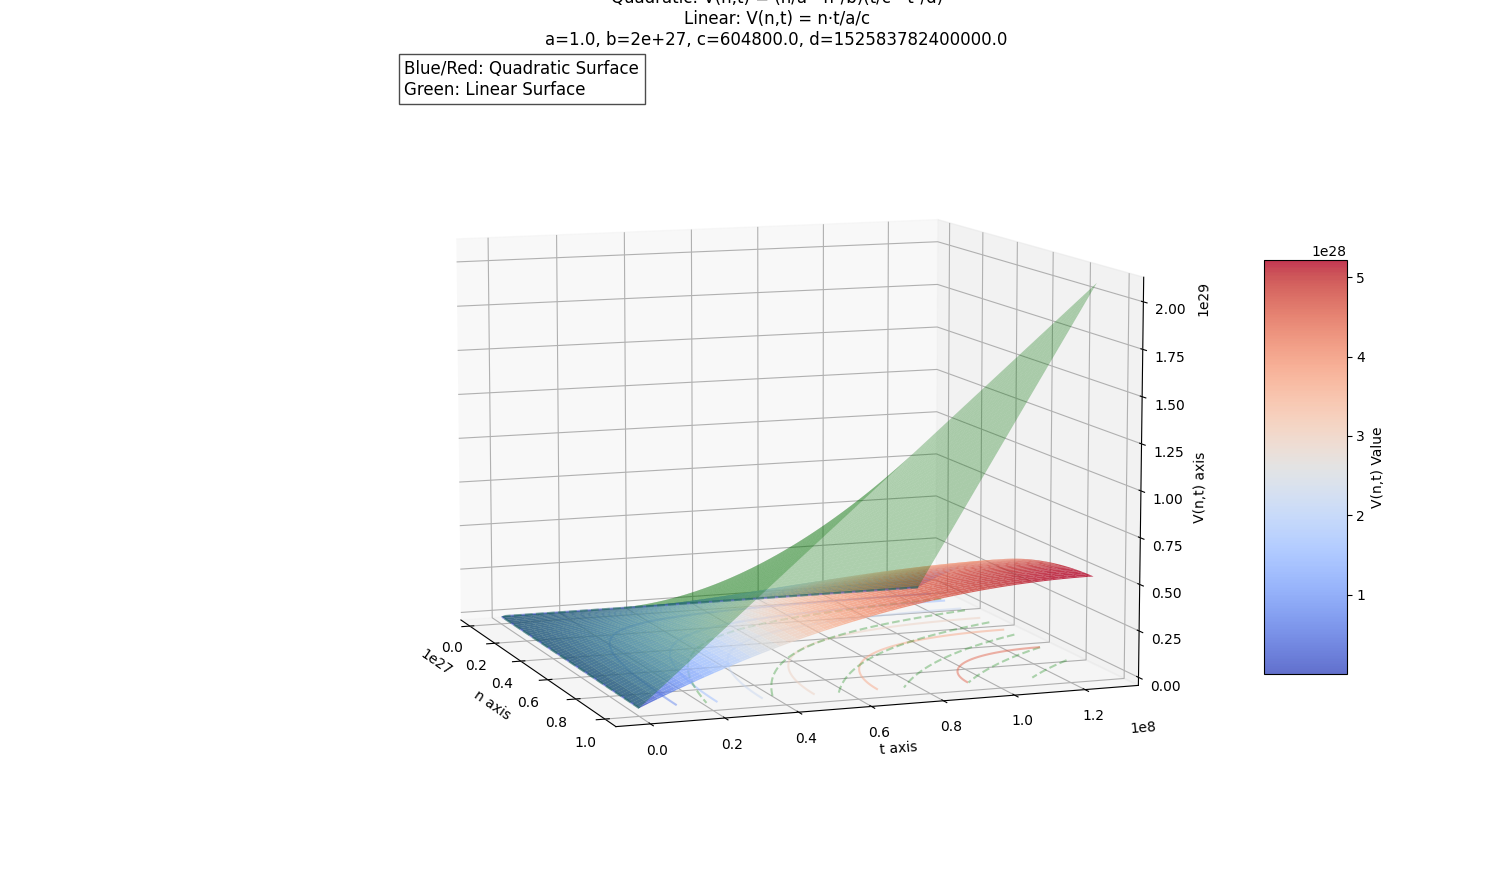
\includegraphics[width=0.7\textwidth]{voting-power-surface.png}
    \caption{An example of $V(n, t)$ with $a = c = 1$ and $b = d = 0.05$ compared with the ``linear surface'' $ab * nt$.}
    \label{fig:example-image}
\end{figure}

If $n$ or $t$ is $0$, $V$ is $0$.
The role of the parameters $b$ and $d$ is to make the voting power sub-linear in $n$ and $t$, respectively.
This means that:
\begin{itemize}
    \item A whale who locks a large amount of tokens does not dominate voting to the same degree as they would in the linear case (e.g. if one user owns 51\% of the tokens, locking them all will result in less than 51\% of the possible voting power).
    \item Locking for the maximum period gets less than double locking for half the maximum period.
    \item The sublinearity can be tuned by changing the value of $b$ and $d$.
      As $b$ or $d$ tends to $0$, the voting power tends to linear in $n$ or $t$ respectively.
\end{itemize}

Voting power decreases as time passes.
Say initial lock is for 100 HYPR for 52 weeks.
Initial voting power is then
\begin{equation}
V(n=100, t=52) = (a\cdot 100 - b\cdot 100^2) \cdot (c\cdot 52 - d\cdot 52^2)
\end{equation}

After one week has past, $t$ declines to $51$.
Each subsequent week, voting power of the locked tokens decreases, until it eventually reaches $0$.

A locked token position can be modified in three ways:
\begin{enumerate}
    \item Token lock can be extended.
       For example, say 100 tokens were locked for 52 weeks and 20 have passed, leaving 32 weeks remaining in the lock.
       The user can extend the lock to 52 weeks once again, extending the lockup period by an additional 20 weeks, and bringing voting power up to its original value.
    \item Tokens may be added.
       For example, say 100 tokens we locked for 52 weeks and 20 have passed, leaving 32 weeks remaining in the lock.
       10 additional tokens might be added, leading to a locked set of 110 tokens for 32 weeks.
    \item Tokens within the locked set may be registered, see \hyperref[sec:registration]{Registration discussion below}.
\end{enumerate}

Note that locked tokens are illiquid (cannot be transferred, or interacted with in any way aside from extending lock; adding tokens; registering locked tokens to Hypermap) until the lock time has passed!

\section{Registration Power}\label{sec:registration}

Tokens that are locked can be registered.
Registration can occur on either all locked tokens (that have not yet been registered) or a subset.
Registration points those tokens at a name-key on the Hypermap.

Registration power has a similar form to voting power.
Registration power depends on two parameters: $n_i$, the number of HYPR tokens registered at name-key $i$, and $t_i$, the remaining period tokens are registered for (in weeks) to name-key $i$.\footnote{
	Recall that the Hypermap has two types of keys, name-keys and data-keys.
	Data-keys hold data, whereas name-keys provide hierarchical structure and can be nested.
	Name-keys can have tokens registered to them to indicate value.
	The registration values found on the Hypermap can be used in arbitrarily programmable ways, with current plans to use them for search and filtering.
	More discussion can be found in the \href{https://hyperware.ai/whitepaper.pdf}{Hyperware Whitepaper}.
}
Tokens must be registered for a duration shorter-than-or-equal-to the tokens are locked for $t_i \leq t$.
The registration power of a wallet for a given name-key is denoted $R(n_i, t_i)$.
\begin{equation}
R(n_i, t_i) = (an_i - bn_i^2) \cdot (ct_i - dt_i^2)
\end{equation}

Each subsequent week, registration power of the locked tokens decreases, until it eventually reaches $0$.
This means that registrations that are not actively updated will naturally decay in relevance, so the Hypermap will be biased towards:
\begin{enumerate}
	\item High value registrations,
	\item Actively updated, long-term registrations.
\end{enumerate}

A registered token position on a given name-key can be modified in two ways:
\begin{enumerate}
    \item Token registration can be extended.
       For example, say 100 tokens were registered for 52 weeks and 20 have passed, leaving 32 weeks remaining in the registration.
       The user can extend the registration to 52 weeks once again, extending the registration period by an additional 20 weeks, and bringing registration power up to its original value.
    \item Tokens may be added.
       For example, say 100 tokens we registered for 52 weeks and 20 have passed, leaving 32 weeks remaining in the registration.
       10 additional tokens might be added, leading to a registered set of 110 tokens for 32 weeks.
\end{enumerate}

Note that registered tokens are illiquid (cannot be transferred, or interacted with in any way aside from extending registration or adding tokens) until the registration time has passed!
Note also that token registration positions expire into a locked token position, and can only become truly liquid once the locked token position expires.
For example, say a user has 100 HYPR.
The use locks 80 HYPR for 52 weeks, so now only has 20 HYPR liquid.
Any of the 80 locked HYPR can be registered for up to 52 weeks.
Say 40 is registered to $foo.os$ for 2 weeks and 30 is registered to $app.bar.os$ for 52 weeks.
Then 10 locked HYPR can still be registered at will.
The $foo.os$ registration will expire after 2 weeks, at which time the state of the locked tokens will look like:
\begin{enumerate}
    \item 50 locked and unregistered, free for registration,
    \item 30 registered for 50 weeks.
\end{enumerate}
After an additional 50 weeks, the $app.bar.os$ registration will expire as will the lock, and the tokens can be unlocked and become liquid again.

\begin{table}[htbp]
    \centering
    \caption{Summary of important known and unknown parameters}
    \label{tab:student-performance}
    \begin{tabular}{|c|c|c|}
    \hline
    \textbf{Parameter} & \textbf{Value} & \textbf{Description} \\
    \hline
    $S$ & $10^9$ & Total token supply \\
    $n_m$ & likely $S$ & Max token parameter in $R$ \\
    $T$ & 4 years = 208 weeks & Max registration time \\
    $a$ & $> 2b \cdot n_m$ & Constraints on $R$'s $n$-dependent parameters \\
    $c$ & $> 2d \cdot T$ & Constraints on $R$'s $t$-dependent parameters \\
    $L_t$ & ? & Vesting lockup duration for team members \\
    $C_t$ & ? & Vesting cliff duration for team members \\
    $L_i$ & ? & Vesting lockup duration for investors \\
    $C_i$ & ? & Vesting cliff duration for investors \\
    \hline
	\end{tabular}
\end{table}

\section{Voting in DAO Governance}\label{sec:voting}

A proposal has a closing time associated with it.
Voters cast votes.
Voting power of voters is calculated at closing time, and the proposal passes or fails.
Voters and their voting power, as well as the result of the vote, is recorded.

\section{Governance Participation Rewards}\label{sec:rewards}

Governance participation incentives are distributed quarterly: 2\% of the incentive treasury per quarter.
For each proposal, $k$, a user $j$ that participates in that vote gets an award $A^{k}_j$ that is a fraction of the incentives dedicated to that vote equal to
\begin{equation}
A^{k}_j = \frac{V^{k}_j}{\sum_j V^{k}_j}
\end{equation}
where $V^{k}_j$ denotes the voting power contributed by user $j$ in the $k$th vote in a quarter.

If no votes occur in a quarter, no incentives are distributed.
If multiple votes occur in a quarter, the incentives are split amongst them based on the total voting power that participated in each vote.
Then the fraction of quarterly incentives allocated to a specific vote $k$, $F^{k}$ is
\begin{equation}
F^{k} = \frac{\sum_j V^{k}_j}{\sum_k \sum_j V^{k}_j}
\end{equation}
and so the total award of a user in a multi-vote quarter becomes
\begin{equation}
A_j = \sum_k \left[F^{k} \cdot A^{k}_j\right]
\end{equation}

Users can delegate their voting power to a third-party.
The delegate's voting power becomes the sum of their own voting power and all voting powers delegated to them
\begin{equation}
V^{(D)}_i = V_i + \sum_j V_j
\end{equation}
Incentive rewards are distributed to the owners of the voting powers, not the delegate.
If the delegate does not cast a vote, the voting power delegated to them earns no rewards from that vote.

\section{Vesting}\label{sec:vesting}

Vesting tokens cannot do anything except be have the vested fraction claimed, depending on the percentage of the vesting time that has passed.
Thus, they cannot participate in registration or governance.
They cannot be transferred.

There are two reasons that vesting tokens cannot participate in registration or governance:
\begin{enumerate}
    \item Simplicity.
         Vesting tokens will only exist for the start of the network.
         There should not be logic for them that lives forever in locking, governance, registration contracts.
    \item Giving community members a headstart on governance and incentive rewards.
         Investors and team members will only be able to access a fraction of their tokens -- the ones that have already vested -- and thus will not be able to control governance due to their outsized ownership in early days.
         This also gives community members a chance to acquire a larger fraction of the governance rewards, improving the distribution of tokens to the community.
         Investors and team members have been of fundamental importance to the project and will continue to be so, but establishing an involved and aligned community is of the utmost importance for Hyperware to succeed.
\end{enumerate}

\section{Open Questions}\label{sec:questions}

\begin{itemize}
    \item Token supply, $S$, is fixed at $10^9$ at launch.
        Will more tokens ever be minted?

        I would recommend: no.
    \item Should the vesting token contract allow an admin (i.e. a Hyperware-held multisig) transfer existing vesting tokens?
        The reason to allow this is in case a vesting token holder loses an account or wants to move funds between, e.g., a hot and cold wallet.
        The reason to disallow this is it gives Hyperware multisig holders the power to arbitrarily change vesting distribution.
        In addition, even in legitimate cases where a user wants to transfer their funds, it puts a huge honus on the admin to confirm the legitimacy of the request.

        I would recommend: no.
    \item ``If no votes occur in a quarter, no incentives are distributed'': see Section~\ref{sec:rewards}.
        Does this lead to bad incentives in either stage of governance?
        E.g., in the initial stage, proposals will be generated by Hyperware, not the DAO (since the DAO will not exist yet).
        Since Hyperware team members will be locked in vesting tokens, the incentive will be for Hyperware to avoid creating proposals in order to delay distribution of incentives until vested.

        After the DAO is in charge of proposing, will quarters in which no useful proposals are put forward incentivize a ``no action'' proposal to force distribution of funds for that quarter?
        
        One way to avoid this is to simply make a ``no-vote quarter'' distribute funds according to voting power at end of quarter (as if all voting power had participated in a vote).
        Another possibility is to accumulate the incentive rewards for that ``no-vote quarter'' and distribute them in the next ``voting quarter''.
        E.g., if three quarters pass without a vote, and in the fourth quarter a vote occurs, that vote will pay out the incentive rewards for all four of those quarters.
\end{itemize}

\end{document}